\documentclass[crop,tikz]{standalone}

%The idea behind this file is that it will be used to store all the maths-related macros that I concoct; so that I can import all the commands by \input{this file} in the preamble of any file that I want to use them in.
%This should make the top-level files look a lot cleaner, and the preamble much shorter!

\usepackage{amssymb}
\usepackage{amsmath}
%\usepackage{mathtools}

%begin the macros via newcommand. Try to group them up reasonably!

%standard sets
\newcommand{\naturals}{\mathbb{N}}			%natural numbers
\newcommand{\integers}{\mathbb{Z}}			%integers
\newcommand{\rationals}{\mathbb{Q}}			%rational numbers
\newcommand{\reals}{\mathbb{R}}				%real numbers
\newcommand{\complex}{\mathbb{C}}			%complex numbers

%brackets and norms
\newcommand{\bracs}[1]{\left( #1 \right)}				%encloses input in brackets
\newcommand{\sqbracs}[1]{\left[ #1 \right]}				%encloses input in square brackets
\newcommand{\clbracs}[1]{\left\{ #1 \right\}}			%encloses input in curly bracers
\newcommand{\abs}[1]{\lvert #1 \rvert}					%absolute value
\newcommand{\norm}[1]{\lvert\lvert #1 \rvert\rvert}		%norm 

%function sets
\newcommand{\smooth}[1]{C^{\infty}\bracs{#1}}							%smooth functions
\newcommand{\ltwo}[2]{L^{2}\bracs{#1,\mathrm{d}#2}}						%general L^2 space
\newcommand{\gradSob}[2]{H^1_\mathrm{grad}\bracs{#1, \mathrm{d}#2}}		%gradient Sobolev space
\newcommand{\curlSob}[2]{H^1_\mathrm{curl}\bracs{#1, \mathrm{d}#2}}		%curl Sobolev space
\newcommand{\kSob}[2]{H^1_{k,\mathrm{curl}}\bracs{#1, \mathrm{d}#2}}	%k-curl Sobolev space
\newcommand{\supp}{\mathrm{supp}}										%support of a function

%grad and curl sets
\newcommand{\gradZero}[2]{\mathcal{G}_{ #1, \mathrm{d}#2}\bracs{0}}		%gradients of zero for domain #1 with measure #2
\newcommand{\curlZero}[2]{\mathcal{C}_{ #1, \mathrm{d}#2}\bracs{0}}	%curls of zero for domain #1 with measure #2
\newcommand{\kcurlZero}[2]{\mathcal{C}_{ #1, \mathrm{d}#2}^{(k)}\bracs{0}}	%k-curls of zero for domain #1 with measure #2

%derivatives and grad-like symbols
\newcommand{\diff}[2]{\dfrac{\mathrm{d}#1}{\mathrm{d}#2}}			%complete derivative d#1/d#2
\newcommand{\pdiff}[2]{\dfrac{\partial #1}{\partial #2}}			%partial derivative p#1/p#2
\newcommand{\ddiff}[2]{\dfrac{\mathrm{d}^2 #1}{\mathrm{d}^2 #2}}	%2nd deriv
\newcommand{\grad}{\nabla}											%grad operator
\newcommand{\curl}[1]{\grad^{(#1)}\wedge}							%curl with superscript #1
\newcommand{\kcurl}[1]{\grad_{#1}^{(k)}\wedge}						%k-curl with measure subscript #1

%displaying integrals
\newcommand{\integral}[3]{\int_{#1}#2 \ \mathrm{d}#3}			%integral, domain #1, integrand #2, measure #3
\newcommand{\md}{\ \mathrm{d}}									%differential d

%convergence
%\newcommand{\lconv}[1]{\xrightarrow{#1}}							%convergence with #1 above the rightarrow - requires mathtools
\newcommand{\lconv}[1]{\overset{#1}{\longrightarrow}}				%convergence with #1 above the rightarrow
\newcommand{\toInfty}[1]{ \ \text{as} \ #1 \rightarrow\infty}		%writes out "as #1 tends to infty"

%notation and variable use throughout the file
\renewcommand{\vec}[1]{\mathbf{#1}}				%vectors are bold, not overline arrow
\newcommand{\recip}[1]{\frac{1}{#1}}			%fast reciprocal as a fraction

\newcommand{\dddom}{\widetilde{\Omega}}			%3D domain notation
\newcommand{\ddom}{\Omega}						%2D domain notation
\newcommand{\dddmes}{\widetilde{\mu}}			%3D measure
\newcommand{\ddmes}{\mu}						%2D measure

\newcommand{\graph}{\mathbb{G}}					%graph variable

\usepackage[utf8]{inputenc}

% 'crop' is the default for v1.0, before it was 'preview'
%\usetikzlibrary{...}% tikz package already loaded by 'tikz' option

\begin{document}

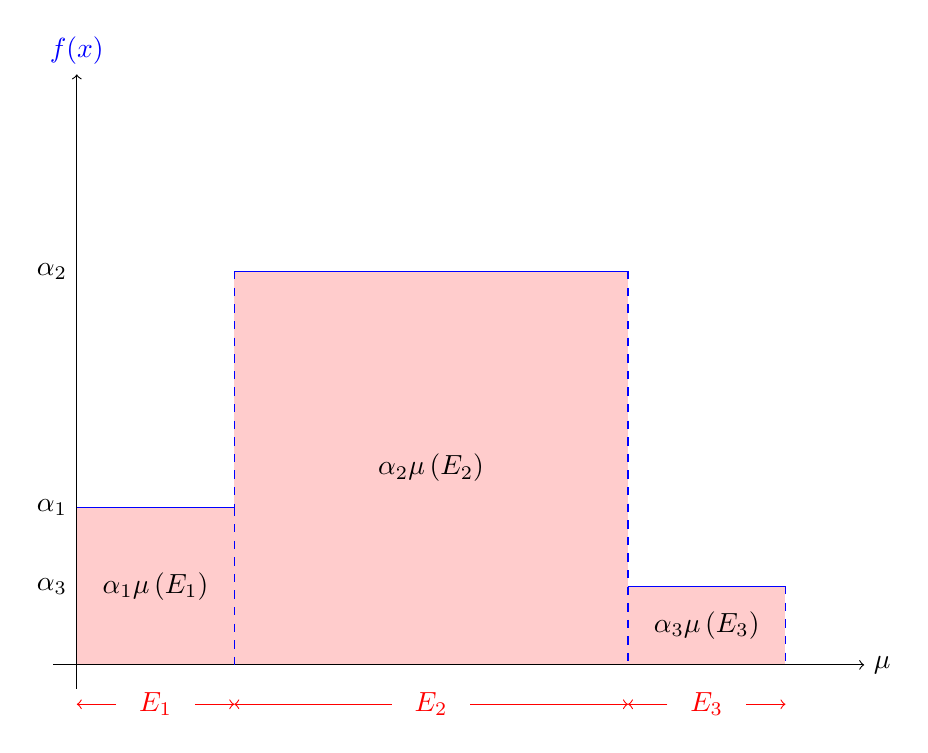
\begin{tikzpicture}

	%division of the range
	\draw[draw=none, fill=red!20!white] (0,0) rectangle (2,2);
	\node[align=center] at (1,1) {$\alpha_1\mu\bracs{E_1}$};
	\draw[draw=none, fill=red!20!white] (2,0) rectangle (7,5);
	\node[align=center] at (4.5,2.5) {$\alpha_2\mu\bracs{E_2}$};
	\draw[draw=none, fill=red!20!white] (7,0) rectangle (9,1);
	\node[align=center] at (8,0.5) {$\alpha_3\mu\bracs{E_3}$};

	\draw[->] (-0.3,0) -- (10,0) node[anchor=west] {$\mu$};
	\draw[->] (0,-0.3) -- (0,7.5);
	\node[anchor=south, color=blue] at (0,7.5) {$f(x)$};
	
	%simple function
	\draw[blue] (0,2) -- (2,2);
	\draw[blue, dashed] (2,2) -- (2,0);
	\node[anchor=east] at (0,2) {$\alpha_1$};
	\draw[blue] (2,5) -- (7,5);
	\draw[blue, dashed] (7,5) -- (7,0);
	\draw[blue, dashed] (2,5) -- (2,2);
	\node[anchor=east] at (0,5) {$\alpha_2$};
	\draw[blue] (7,1) -- (9,1);
	\draw[blue, dashed] (9,1) -- (9,0);
	\draw[blue, dashed] (7,5) -- (7,1);
	\node[anchor=east] at (0,1) {$\alpha_3$};
	
	%\mu-axis labels
	\draw[->, red] (1-0.5,-0.5) -- (0,-0.5); 
	\draw[->, red] (1+0.5,-0.5) -- (2,-0.5);
	\node[align=center, red] at (1,-0.5) {$E_1$};
	\draw[->, red] (4.5-0.5,-0.5) -- (2,-0.5); 
	\draw[->, red] (4.5+0.5,-0.5) -- (7,-0.5);
	\node[align=center, red] at (4.5,-0.5) {$E_2$};
	\draw[->, red] (8-0.5,-0.5) -- (7,-0.5); 
	\draw[->, red] (8+0.5,-0.5) -- (9,-0.5);
	\node[align=center, red] at (8,-0.5) {$E_3$};

\end{tikzpicture}

\end{document}